\documentclass[11pt]{article}
\usepackage{graphicx} % Required for inserting images
\usepackage{amsmath,mathtools}
\usepackage{float}
\usepackage{ragged2e}
\usepackage[none]{hyphenat}

\usepackage{newtxtext, newtxmath}

\usepackage[spanish]{babel}
\usepackage[utf8]{inputenc}
\usepackage[backend=biber]{biblatex}
\bibliography{referencias}

\usepackage{tikz}
\usetikzlibrary{mindmap}

\usepackage{circuitikz}
\ctikzset{bipoles/thickness=1.2}
\usetikzlibrary{shapes,arrows}

\usepackage{pgfplots}
\pgfplotsset{width=10cm,compat=newest}

\usepackage[
paperwidth=6in,
  paperheight=9in,
  top=0.45in,
  bottom=0.90in,
  left=1.0in,
  right=0.80in,
  headheight=13.6pt
]{geometry}


%Configuracion para las paginas%
\pagestyle{fancy}
\fancyhf{}
\lhead{\thepage}
\setcounter{page}{215}

\renewcommand{\headrulewidth}{0pt}

\title{
  \normalsize CAPITULO 5
  \vspace{0.5cm}
  \begin{center}
    \large CHANGE
  \end{center}
  }
\date{}

\begin{document}

\maketitle
\thispagestyle{empty}
\vspace{-1cm}

\begin{justifying}
  \noindent 
  Hasta ahora no hemos abordado el cambio. Pero, si creemos en la ciencia, debemos defender el postulado ontológico de que todo 
  está en constante cambio. De hecho, las ciencias describen, explican, predicen, 
  controlan o provocan cambios de diversos tipos, como el movimiento, la acreción, 
  la división y la evolución. Por lo tanto, la ontología debería analizar y sistema tizar estos diversos tipos de cambio.

  Mientras algunos metafísicos se han dedicado a elogiar el cambio, otros lo han negado y ninguno lo ha descrito correctamente. Nos esforzaremos por construir un concepto de cambio lo suficientemente amplio y, por lo tanto, lo suficientemente pobre como para abarcar todos los conceptos de cambio, en particular los que se dan en las ciencias, y esbozar teorías generales del cambio de algunos tipos típicos. Estos son los objetivos del presente capítulo, dedicado al cambio en general. El tema del cambio cualitativo se abordará en el volumen complementario, \textit{Un Mundo de Sistemas}.

  Un cambio es un evento o un proceso, ya sea cuantitativo, cualitativo o ambos. Sea cual sea su naturaleza, un cambio es una modificación en o de alguna cosa o cosas: más precisamente, consiste en una variación del estado de una entidad. Dicho de forma negativa, no existe cambio separado de las cosas; ni, de hecho, existen cosas inmutables, aunque algunas cambien lentamente o solo en ciertos aspectos limitados. El mundo, entonces, consiste en cosas que no permanecen en el mismo estado para siempre. Esta hipótesis metafísica es una extrapolación tanto de la experiencia ordinaria como del conocimiento científico. La hipótesis contraria, que nada cambia, es una extravagancia filosófica poco digna de la consideración de una persona cuerda.

\end{justifying}





\begin{justifying}
	\noindent Conocimiento de la naturaleza de la cosa en cuestión: por lo tanto,
	es idealmente adecuado para la ontología o la teoría general de las cosas.
	Comencemos entonces recordando brevemente las nociones de estado y espacio de estados,
	para adentrarnos inmediatamente al fondo del asunto.

	\section{\centering \large CAMBIABILIDAD}
	\subsection{Preliminares}
	\noindent Todo se encuentra en un estado u otro en relación con un marco de referencia determinado.
	Y cada estado (relativo) de una cosa viene determinado de forma única por las
	propiedades de esta última (en relación con algún marco). Por lo tanto, el estado de una cosa
	con n propiedades, cada una representada por una función (de estado), es una n-tupla de
	valores de las funciones que representan esas propiedades. Los diferentes estados
	corresponden a (están representados por) diferentes n-tuplas. Un cambio en la
	representación de las propiedades, o en la elección del marco de referencia, da lugar a
	una representación diferente de los estados. Esto demuestra que nuestro conocimiento de
	un estado depende en parte de nosotros mismos y del estado de la técnica, pero no
	de que el estado en sí mismo sea un artefacto del observador. En resumen, los estados
	son relativos.

	Pretend, for the sake of definiteness, that a certain thing x, such as a
	camera shutter or an electrical switch, has a single dichotomic general
	property: that it is either open (1) or closed (0). The possible states of x
	are then 0 and 1. In other words, the state space of x is S(x)={O, I}.
	Actually this is an extreme oversimplification: 0 and 1 are just the states
	of interest for some definite purposes. Any real thing has a large number
	n of properties Pi' each representable by a function Fj, where 1 ~ i ~ n.
	The possible degrees or intensities of property Pi are represented as so
	many values of the function Fj. Hence the conceivable state space of the
	thing will be the cross product of the images of these functions. And the
	nomological state space will be a subset of the fonner space, resulting
	from the laws involving the Pi: see Figure 5.1. All of this holds, of
	course, for a given representation of properties, hence states.


	\begin{center}
		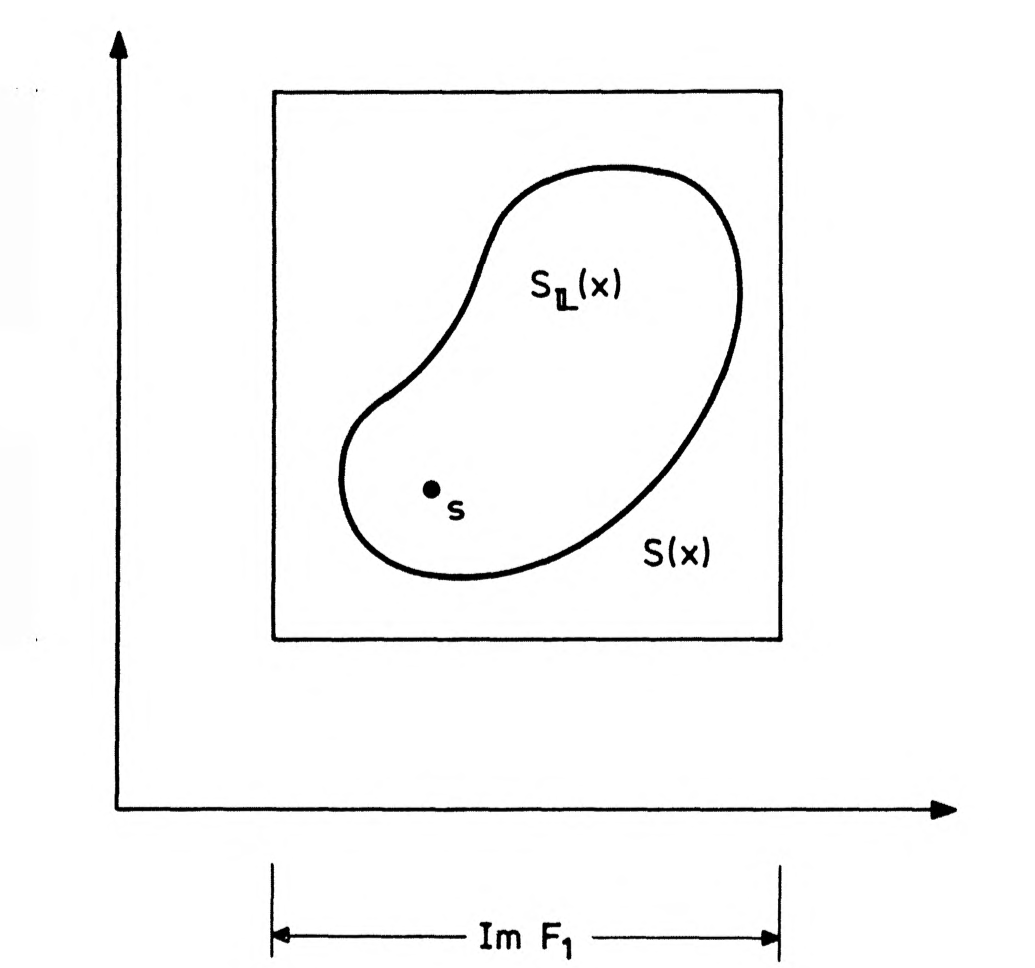
\includegraphics[width=0.6\textwidth]{img/Figura5-1.png}
		\\ \scriptsize Fig. 5.l. El espacio de estados concebible $S(x)$ y el espacio de estados legítimo $S_\mathrm{L}(x)$ de una cosa $x$
		con dos propiedades representadas por las funciones $F_\mathrm{1}$ y $F_\mathrm{2}$.
		\textit{'$F$'} se lee \textit{'la imagen $F$'} es el conjunto de valores, o rango, de $F$.
	\end{center}


	\noindent la curva con la ayuda de un parámetro, cuya interpretación estándar es el tiempo.
	Pero una de las ventajas de la representación del cambio en el espacio de estados
	es que no requiere el uso explícito del concepto de tiempo.

	Para aclarar las ideas, consideremos el espacio de estados del conjunto genético de una población
	de organismos. Ese conjunto está incluido en el espacio cartesiano cuyos ejes son
	las frecuencias genéticas del conjunto. Cada punto de este espacio representa un estado posible del conjunto genético. El punto representativo, el que representa el estado real del sistema, permanecerá fijo solo si los organismos no sufren mutaciones, lo que nunca ocurre, ni siquiera si el entorno de la población es muy estable, como una laguna tropical.
	De lo contrario, el punto representativo se mueve (en el espacio de estados, no en el espacio ordinario) describiendo una trayectoria. Esta curva, que en el caso de la evolución biológica no tiene bucles, representa la historia genética del conjunto genético.
	De lo contrario, el punto representativo se mueve (en el espacio de estados, no en el espacio ordinario)
	describiendo una trayectoria. Esta curva, que en el caso de la
	evolución biológica no tiene bucles , representa la historia genética del
	pool genético, o la evolución de la población correspondiente a nivel genético.
	Cualquier segmento de la historia total puede denominarse evento o
	proceso que involucra al pool genético. (Véase la figura 5.2).

	\begin{center}
		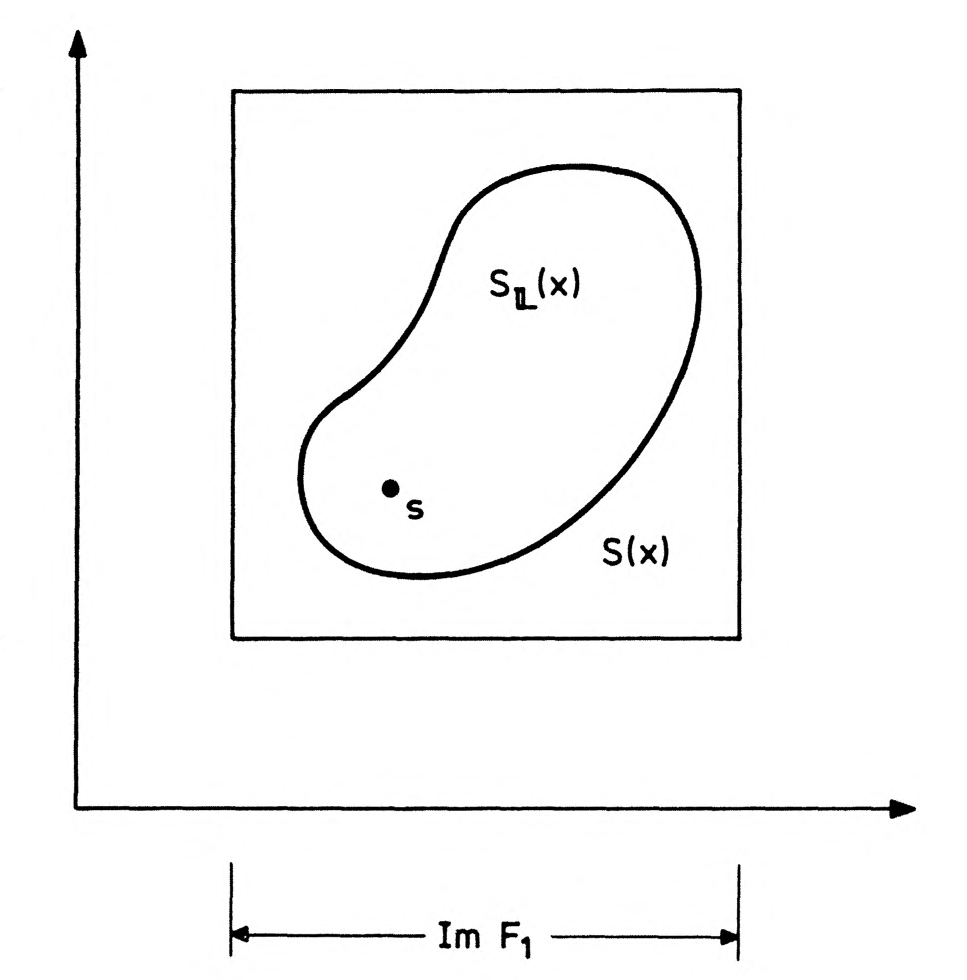
\includegraphics[width=0.6\textwidth]{img/Figura5-2.png}
		\\ \scriptsize Fig. 5.2. El cambio en las frecuencias genéticas en un acervo genético,
		en respuesta a la acción conjunta de la mutación y la selección.
		Los extremos de la curva representan el origen y la extinción de la población dada.
	\end{center}
    Demasiado para un trasfondo intuitivo.

    \subsection{Capacidad de cambio}
    Antes de abordar el cambio real, conviene aclarar la noción intuitiva
    de mutabilidad o variabilidad:

    \begin{quote}
    	\textit{Una cosa es mutable o variable si puede cambiar de estado, es decir,
    	pasar de un estado a otro.}
    \end{quote}
    

\end{justifying}
\begin{justifying}
    Isaac
\end{justifying}
\begin{justifying}
    Miguel 
    Palafox en tanga
\end{justifying}
\begin{justifying}
    Astorga
\end{justifying}
\begin{justifying}
    Esau
\end{justifying}
\begin{justifying}
    Pacheco tryhard lo mejor del mundo
\end{justifying}

\printbibliography


\end{document}